\begin{center}
\begin{minipage}{0.95\linewidth}
\centering
\shorthandoff{<>}
\textbf{Si el observador 1 comienza primero: $T_1\le T_2$}

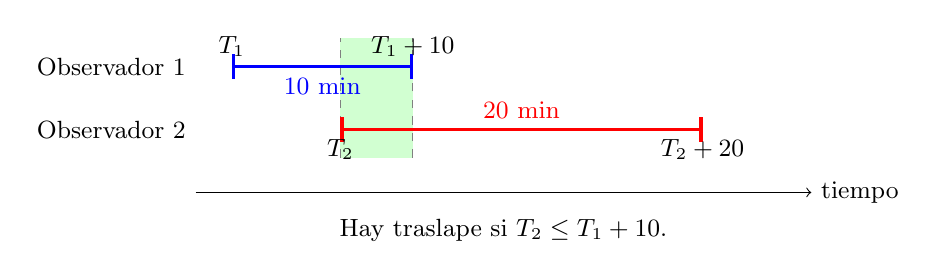
\begin{tikzpicture}[x=0.23cm,y=0.8cm,font=\small]
  \fill[green!18] (16,0.55) rectangle (20,2.45);
  \draw[dashed,gray] (16,0.55) -- (16,2.45);
  \draw[dashed,gray] (20,0.55) -- (20,2.45);
  \node[left] at (8,2) {Observador 1};
  \node[left] at (8,1) {Observador 2};
  \draw[blue,very thick,|-|] (10,2) -- (20,2)
    node[midway,below] {$10$ min};
  \node[above] at (10,2) {$T_1$};
  \node[above] at (20,2) {$T_1+10$};
  \draw[red,very thick,|-|] (16,1) -- (36,1)
    node[midway,above] {$20$ min};
  \node[below] at (16,1) {$T_2$};
  \node[below] at (36,1) {$T_2+20$};
  \draw[->] (8,0) -- (42,0) node[right] {tiempo};
  \node at (25,-0.6) {Hay traslape si $T_2\le T_1+10$.};
\end{tikzpicture}

\medskip
\textbf{Si el observador 2 comienza primero: $T_2\le T_1$}

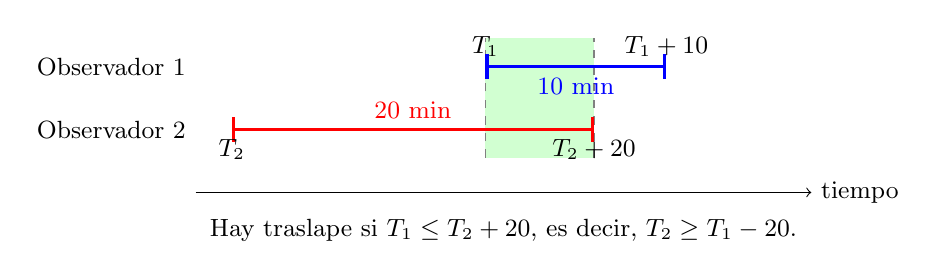
\begin{tikzpicture}[x=0.23cm,y=0.8cm,font=\small]
  \fill[green!18] (24,0.55) rectangle (30,2.45);
  \draw[dashed,gray] (24,0.55) -- (24,2.45);
  \draw[dashed,gray] (30,0.55) -- (30,2.45);
  \node[left] at (8,2) {Observador 1};
  \node[left] at (8,1) {Observador 2};
  \draw[blue,very thick,|-|] (24,2) -- (34,2)
    node[midway,below] {$10$ min};
  \node[above] at (24,2) {$T_1$};
  \node[above] at (34,2) {$T_1+10$};
  \draw[red,very thick,|-|] (10,1) -- (30,1)
    node[midway,above] {$20$ min};
  \node[below] at (10,1) {$T_2$};
  \node[below] at (30,1) {$T_2+20$};
  \draw[->] (8,0) -- (42,0) node[right] {tiempo};
  \node at (25,-0.6) {Hay traslape si $T_1\le T_2+20$, es decir, $T_2\ge T_1-20$.};
\end{tikzpicture}
\shorthandon{<>}

\small La franja verde indica el intervalo común en estos dos ejemplos de traslape. Los segmentos azules duran $10$ minutos y los rojos $20$ minutos; las posiciones de inicio son ilustrativas.
\end{minipage}
\end{center}